\chapter{Pendulums, Oscillators, and Phase Space}

We shall work through three examples. The first is simple, the second is much
more complicated, and the third is simpler again. There is a reason for this
order. The simple and double pendulums show why Lagrange's equations are often
far easier to use than direct force resolution. The harmonic oscillator then
introduces the variables and geometry of Hamiltonian mechanics.

The advantage is elementary but decisive. Newton's equation asks for
accelerations, which are second derivatives. In curvilinear or angular
coordinates, their Cartesian components can become unpleasant. A Lagrangian
calculation ordinarily asks first for velocities, which are only first
derivatives. Once the kinetic and potential energies are known,
\[
 \mathcal L=T-U,
\]
the Euler--Lagrange equations turn the remaining work into a fixed procedure.
If the resulting differential equations resist analytic solution, they can be
integrated numerically. The difficulty of solving a trajectory is separate
from the difficulty of formulating the correct equations.

\section{The Simple Pendulum}

Take a mass \(m\) at the end of a rigid, massless rod of fixed length \(r\).
The rod pivots in a vertical plane. Its only changing coordinate is the angle
\(\theta\), measured from the downward vertical. With horizontal coordinate
\(x\) and downward-positive vertical coordinate \(y\),
\begin{equation}
 x=r\sin\theta,
 \qquad
 y=r\cos\theta.
 \label{eq:l05-pendulum-position}
\end{equation}

\begin{figure}[tbp]
\centering

\includegraphics[width=0.70\textwidth]{lecture_05_figure_01.png}
\caption{The pendulum geometry at 00:05:32. The rod length \(r\), angle
\(\theta\), and horizontal projection \(r\sin\theta\) are complete and
unobstructed.}
\label{fig:l05-pendulum-board}
\end{figure}

Differentiation gives
\begin{equation}
 v_x=r\cos\theta\,\dot\theta,
 \qquad
 v_y=-r\sin\theta\,\dot\theta.
 \label{eq:l05-pendulum-velocity}
\end{equation}
The two trigonometric factors disappear when the speed is squared:
\begin{align}
 v^2
 &=v_x^2+v_y^2 \notag\\
 &=r^2\dot\theta^2
   \left(\cos^2\theta+\sin^2\theta\right)
 =r^2\dot\theta^2.
\end{align}
Hence
\begin{equation}
 T=\frac12mr^2\dot\theta^2.
 \label{eq:l05-pendulum-T}
\end{equation}

Only differences of gravitational potential matter. Taking zero potential
when the rod is horizontal, the bob's height relative to the pivot is
\(-r\cos\theta\), so
\begin{equation}
 U=-mgr\cos\theta.
 \label{eq:l05-pendulum-U}
\end{equation}
At \(\theta=0\) the bob is at the bottom and \(U=-mgr\); at
\(\theta=\pi\) it is upright and \(U=+mgr\).

The Lagrangian is therefore
\begin{equation}
 \boxed{\mathcal L
 =\frac12mr^2\dot\theta^2+mgr\cos\theta.}
 \label{eq:l05-pendulum-L}
\end{equation}

\begin{classroomqa}
\audiencequestion{Why does the Lagrangian contain
\(+mgr\cos\theta\) when gravity pulls downward?}
\lecturerresponse{The potential itself is
\(U=-mgr\cos\theta\) in the chosen convention, and the Lagrangian is
\(\mathcal L=T-U\). Subtracting this negative potential produces the plus
sign. The force will acquire the expected restoring sign when
\(\mathcal L\) is differentiated with respect to \(\theta\).}
\end{classroomqa}

\begin{figure}[tbp]
\centering

\includegraphics[width=0.76\textwidth]{lecture_05_figure_02.png}
\caption{The completed kinetic energy, potential energy, and pendulum
Lagrangian at 00:10:50. The gesture emphasizes the plus sign created by
subtracting the negative gravitational potential.}
\label{fig:l05-pendulum-lagrangian}
\end{figure}

\subsection{Equation of motion}

The momentum conjugate to \(\theta\) is
\begin{equation}
 \pi_\theta
 =\frac{\partial\mathcal L}{\partial\dot\theta}
 =mr^2\dot\theta.
 \label{eq:l05-pendulum-momentum}
\end{equation}
It is the angular momentum about the pivot, although the derivation needs only
its definition. The Euler--Lagrange equation gives
\begin{equation}
 \frac{d}{dt}\left(mr^2\dot\theta\right)
 =-mgr\sin\theta,
\end{equation}
or
\begin{equation}
 \boxed{\ddot\theta+\frac{g}{r}\sin\theta=0.}
 \label{eq:l05-pendulum-eom}
\end{equation}
This nonlinear equation can be integrated directly on a computer by advancing
\(\theta\) and \(\dot\theta\) over short time steps.

\begin{figure}[tbp]
\centering

\includegraphics[width=0.78\textwidth]{lecture_05_figure_03.png}
\caption{The completed pendulum Euler--Lagrange equation at 00:12:27. The
upper board retains the Lagrangian from which the lower equation follows.}
\label{fig:l05-pendulum-eom}
\end{figure}

\subsection{Hamiltonian and energy}

There is one generalized coordinate, so the Hamiltonian is
\begin{align}
 H
 &=\pi_\theta\dot\theta-\mathcal L \notag\\
 &=mr^2\dot\theta^2
 -\left(\frac12mr^2\dot\theta^2+mgr\cos\theta\right) \notag\\
 &=\frac12mr^2\dot\theta^2-mgr\cos\theta.
 \label{eq:l05-pendulum-H}
\end{align}
It is exactly \(T+U\), as expected.

\begin{classroomqa}
\audiencequestion{Should
\(\sum_i\pi_i\dot q_i\) always equal \(2T\)?}
\lecturerresponse{It does for the ordinary kinetic energies used here. If
\(T\) is homogeneous of degree two in the generalized velocities, Euler's
homogeneous-function theorem gives
\(\sum_i(\partial T/\partial\dot q_i)\dot q_i=2T\).
It is not a universal identity for every possible Lagrangian, so it should be
checked rather than assumed.}
\end{classroomqa}

\section{The Pendulum Energy Landscape}

We do not need the exact nonlinear solution to classify the motion. The
potential changes by
\begin{equation}
 U(\pi)-U(0)=mgr-(-mgr)=2mgr
 \label{eq:l05-pendulum-barrier}
\end{equation}
between the bottom and the upright position.

Suppose the pendulum starts at the bottom with a push. If its initial kinetic
energy is less than \(2mgr\), it spends that energy climbing, reaches a
turning point with \(\dot\theta=0\), and returns. It oscillates between two
turning points. If the kinetic energy exceeds \(2mgr\), some remains when the
bob passes the upright point, and the pendulum continues to rotate. The
rotation may be clockwise or counterclockwise. Exactly at the threshold, the
ideal trajectory approaches the unstable upright configuration with zero
speed. This separatrix motion is possible but requires exact tuning.

\begin{classroomqa}
\audiencequestion{What is meant by the \emph{top} of the orbit? Is it the
ceiling?}
\lecturerresponse{The pivot is imagined to permit a complete \(360^\circ\)
rotation. The top is the configuration \(\theta=\pi\), with the bob vertically
above the pivot. The phrase does not refer to a physical ceiling obstructing
the rod.}
\end{classroomqa}

Thus the familiar swinging pendulum and the continuously rotating pendulum
are different families of motion separated by the threshold energy. This
qualitative conclusion follows immediately from conservation of
Eq.~\eqref{eq:l05-pendulum-H}.

\section{The Double Pendulum}

The single pendulum is simple enough that direct force resolution remains
possible. The double pendulum is the real test. Its motion can become chaotic,
and resolving all rod tensions and accelerations by \(F=ma\) is treacherous.
The Lagrangian method, by contrast, changes only the amount of algebra.

Take two equal point masses \(m\) joined by two massless rods of equal length
\(r\), moving in one vertical plane. Let \(\theta\) be the angle of the first
rod from the downward vertical and let \(\phi\) be the angle of the second rod
from the same vertical.

\begin{classroomqa}
\audiencequestion{Must the double pendulum remain in one plane?}
\lecturerresponse{No. A spatial double pendulum is a legitimate problem, but
it needs more coordinates. We choose planar motion here so that the two angles
\(\theta\) and \(\phi\) form a minimal complete set.}
\end{classroomqa}

\begin{figure}[tbp]
\centering
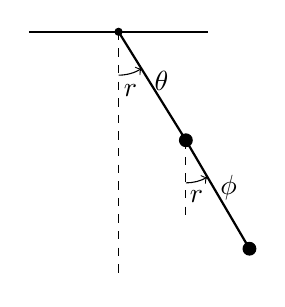
\begin{tikzpicture}[scale=0.95]
\draw[thick] (-1.2,0) -- (1.2,0);
\fill (0,0) circle (0.055);
\draw[dashed] (0,0) -- (0,-3.3);
\draw[thick] (0,0) -- (0.9,-1.45);
\filldraw (0.9,-1.45) circle (0.085);
\draw[thick] (0.9,-1.45) -- (1.75,-2.90);
\filldraw (1.75,-2.90) circle (0.085);
\draw[thin,->] (0,-0.58) arc (-90:-58:0.58);
\draw[dashed] (0.9,-1.45) -- (0.9,-2.55);
\draw[thin,->] (0.9,-2.02) arc (-90:-60:0.57);
\node[right] at (0.35,-0.66) {\(\theta\)};
\node[right] at (1.23,-2.08) {\(\phi\)};
\node[left] at (0.38,-0.78) {\(r\)};
\node[left] at (1.26,-2.20) {\(r\)};
\end{tikzpicture}
\caption{Both angles are measured from the same vertical direction. This
choice makes a common rotation appear as equal shifts of \(\theta\) and
\(\phi\).}
\label{fig:l05-double-geometry}
\end{figure}

The first mass has kinetic energy
\begin{equation}
 T_1=\frac12mr^2\dot\theta^2.
\end{equation}
The second mass moves both because the first mass moves and because the second
rod rotates relative to the first mass. Its velocity components are
\begin{align}
 v_{2x}
 &=r\cos\theta\,\dot\theta+r\cos\phi\,\dot\phi,\\
 v_{2y}
 &=-r\sin\theta\,\dot\theta-r\sin\phi\,\dot\phi.
 \label{eq:l05-lower-velocity}
\end{align}

\begin{figure}[tbp]
\centering

\includegraphics[width=0.82\textwidth]{lecture_05_figure_06.png}
\caption{The two contributions to the lower bob's velocity at 00:29:02.
Each Cartesian component contains motion inherited from the upper bob and
motion due to the second rod.}
\label{fig:l05-double-velocity}
\end{figure}

Squaring and adding produces two diagonal terms and one mixed term:
\begin{align}
 v_2^2
 ={}&r^2\dot\theta^2+r^2\dot\phi^2 \notag\\
 &+2r^2\dot\theta\dot\phi
 \left(\cos\theta\cos\phi+\sin\theta\sin\phi\right).
\end{align}
The trigonometric identity
\begin{equation}
 \cos\theta\cos\phi+\sin\theta\sin\phi
 =\cos(\theta-\phi)
 \label{eq:l05-angle-identity}
\end{equation}
then gives
\begin{equation}
 T_2=\frac12mr^2\dot\theta^2
 +\frac12mr^2\dot\phi^2
 +mr^2\dot\theta\dot\phi\cos(\theta-\phi).
\end{equation}
Adding the first bob,
\begin{equation}
 \boxed{
 T=mr^2\dot\theta^2
 +\frac12mr^2\dot\phi^2
 +mr^2\dot\theta\dot\phi\cos(\theta-\phi).}
 \label{eq:l05-double-T}
\end{equation}

\begin{classroomqa}
\audiencequestion{Why did the factor \(1/2\) disappear from the
\(\dot\theta^2\) term?}
\lecturerresponse{Both masses carry the motion generated by the first rod.
The upper bob contributes \(\tfrac12mr^2\dot\theta^2\), and the lower bob
contributes another identical term. Their sum is
\(mr^2\dot\theta^2\). The simple coefficient depends on our choice of equal
masses and equal rod lengths.}
\end{classroomqa}

The gravitational energy must also count the first rod twice, because both
masses rise when \(\theta\) changes:
\begin{align}
 U
 &=-mgr\cos\theta
 -mg(r\cos\theta+r\cos\phi) \notag\\
 &=-2mgr\cos\theta-mgr\cos\phi.
 \label{eq:l05-double-U}
\end{align}

\begin{classroomqa}
\audiencequestion{Are the two gravitational energies measured from the same
reference point?}
\lecturerresponse{Yes. The lower bob's vertical coordinate is the sum of the
two rod projections. Its energy therefore includes both
\(-mgr\cos\theta\) and \(-mgr\cos\phi\), while the upper bob supplies a
second \(-mgr\cos\theta\). A common additive constant would still be
irrelevant.}
\end{classroomqa}

The full Lagrangian is
\begin{equation}
 \boxed{
 \mathcal L=
 mr^2\dot\theta^2
 +\frac12mr^2\dot\phi^2
 +mr^2\dot\theta\dot\phi\cos(\theta-\phi)
 +mgr(2\cos\theta+\cos\phi).}
 \label{eq:l05-double-L}
\end{equation}
Nothing was guessed. We chose coordinates, differentiated positions, formed
\(T\) and \(U\), and subtracted.

\begin{figure}[tbp]
\centering

\includegraphics[width=0.84\textwidth]{lecture_05_figure_04.png}
\caption{The double-pendulum kinetic energy, potential energy, Lagrangian, and
common angle shift at 00:52:47. The board preserves the
\(\cos(\theta-\phi)\) coupling that controls the later derivatives.}
\label{fig:l05-double-lagrangian}
\end{figure}

\section{Rotation Symmetry Without Gravity}

Gravity singles out the vertical direction, so the full Lagrangian
Eq.~\eqref{eq:l05-double-L} is not invariant under a common planar rotation.
Now imagine the apparatus far from a gravitational field. Removing the last
two potential terms leaves
\begin{equation}
 \mathcal L_0=
 mr^2\dot\theta^2
 +\frac12mr^2\dot\phi^2
 +mr^2\dot\theta\dot\phi\cos(\theta-\phi).
 \label{eq:l05-double-free-L}
\end{equation}
It is invariant under
\begin{equation}
 \theta\longmapsto\theta+\epsilon,
 \qquad
 \phi\longmapsto\phi+\epsilon.
 \label{eq:l05-common-rotation}
\end{equation}
Adding a constant changes neither angular velocity, and the difference
\(\theta-\phi\) remains fixed.

\begin{classroomqa}
\audiencequestion{Why does the coupling contain only
\(\theta-\phi\), rather than \(\theta+\phi\)?}
\lecturerresponse{Without gravity there is no absolute direction in the
plane. A common rotation must leave the kinetic energy unchanged.
\(\theta-\phi\) is invariant under that rotation, whereas
\(\theta+\phi\) changes by \(2\epsilon\). The trigonometric identity in
Eq.~\eqref{eq:l05-angle-identity} is therefore also a visible statement of
rotational symmetry.}
\end{classroomqa}

For this symmetry the two generators are both \(1\). Noether's charge is
\begin{equation}
 Q=\pi_\theta+\pi_\phi.
 \label{eq:l05-double-Q}
\end{equation}
The mixed kinetic term makes each canonical momentum depend on both angular
velocities:
\begin{align}
 \pi_\theta
 &=2mr^2\dot\theta
 +mr^2\dot\phi\cos(\theta-\phi),\\
 \pi_\phi
 &=mr^2\dot\phi
 +mr^2\dot\theta\cos(\theta-\phi).
 \label{eq:l05-double-momenta}
\end{align}
Thus
\begin{equation}
 \boxed{
 Q=mr^2\left[
 2\dot\theta+\dot\phi
 +(\dot\theta+\dot\phi)\cos(\theta-\phi)
 \right]=\text{constant}.}
 \label{eq:l05-double-charge}
\end{equation}
This is the total angular momentum. Once its initial value is known, one
relation among the velocities remains fixed throughout the motion.

\begin{figure}[tbp]
\centering

\includegraphics[width=0.88\textwidth]{lecture_05_figure_07.png}
\caption{The two canonical momenta and their conserved sum at 00:46:15.
The mixed velocity dependence is complete and unobstructed.}
\label{fig:l05-double-charge}
\end{figure}

\subsection{The coupled equations}

The equations may be unpleasant, but their construction is unambiguous:
\begin{equation}
 \frac{d}{dt}\frac{\partial\mathcal L}{\partial\dot\theta}
 =\frac{\partial\mathcal L}{\partial\theta},
 \qquad
 \frac{d}{dt}\frac{\partial\mathcal L}{\partial\dot\phi}
 =\frac{\partial\mathcal L}{\partial\phi}.
 \label{eq:l05-double-EL}
\end{equation}
Expanding Eq.~\eqref{eq:l05-double-L} carefully, with
\(\Delta=\theta-\phi\), gives the useful implicit pair
\begin{align}
 2\ddot\theta+\ddot\phi\cos\Delta
 +\dot\phi^2\sin\Delta
 +2\frac{g}{r}\sin\theta&=0,\\
 \ddot\phi+\ddot\theta\cos\Delta
 -\dot\theta^2\sin\Delta
 +\frac{g}{r}\sin\phi&=0.
 \label{eq:l05-double-expanded}
\end{align}
Setting \(g=0\) recovers the rotation-invariant case.

\begin{classroomqa}
\audiencequestion{When differentiating
\(\cos(\theta-\phi)\), where do the opposite signs enter?}
\lecturerresponse{A partial derivative with respect to \(\theta\) gives
\(-\sin(\theta-\phi)\), while a partial derivative with respect to \(\phi\)
gives \(+\sin(\theta-\phi)\). A time derivative also differentiates both
angles:
\[
 \frac{d}{dt}\cos(\theta-\phi)
 =-\sin(\theta-\phi)(\dot\theta-\dot\phi).
\]
Keeping partial and total derivatives distinct removes the apparent
ambiguity.}
\end{classroomqa}

The energy is obtained by reversing the sign of the potential contribution:
\begin{equation}
 E=T+U
 =mr^2\dot\theta^2+\frac12mr^2\dot\phi^2
 +mr^2\dot\theta\dot\phi\cos\Delta
 -mgr(2\cos\theta+\cos\phi).
\end{equation}
Without gravity, energy and \(Q\) provide two conserved relations. They do not
make the trajectories visually simple, but they substantially reduce the
problem. This is the desired lesson: difficult mechanics can still be reduced
to a reliable algorithm.

\section{Why Harmonic Motion Is Universal}

We now turn to the most basic nontrivial problem in theoretical physics. A
free particle is simpler, but the harmonic oscillator is the structure that
reappears whenever a stable system is disturbed slightly from equilibrium.
The pendulum already contains it.

Near \(\theta=0\),
\begin{equation}
 U(\theta)=-mgr\cos\theta
 =-mgr+\frac12mgr\,\theta^2
 -\frac1{24}mgr\,\theta^4+\cdots.
 \label{eq:l05-pendulum-expansion}
\end{equation}
The constant \(-mgr\) has no effect on the equations of motion. To quadratic
order,
\begin{equation}
 \mathcal L
 \simeq
 \frac12mr^2\dot\theta^2-\frac12mgr\,\theta^2,
\end{equation}
which is the Lagrangian of a harmonic oscillator.

\begin{figure}[tbp]
\centering

\includegraphics[width=0.82\textwidth]{lecture_05_figure_08.png}
\caption{The exact pendulum potential and its quadratic approximation at
00:59:15. The parabola agrees with the cosine potential near the stable
minimum and departs from it for larger angles.}
\label{fig:l05-potential-board}
\end{figure}

\begin{classroomqa}
\audiencequestion{What happened to the constant \(-mgr\)?}
\lecturerresponse{It remains in the numerical value assigned to the energy,
but it has zero derivative. Adding or subtracting a constant from
\(\mathcal L\) changes neither Euler--Lagrange equation. We may choose the
zero of potential for convenience.}
\end{classroomqa}

The canonical realization is a mass on a spring. Let \(x=0\) be its equilibrium
position and write
\begin{equation}
 U(x)=\frac12kx^2,
 \qquad
 \mathcal L=\frac12m\dot x^2-\frac12kx^2.
 \label{eq:l05-oscillator-L}
\end{equation}
The force is
\begin{equation}
 F=-\frac{dU}{dx}=-kx,
\end{equation}
which is Hooke's law. Positive displacement produces a negative force and
negative displacement produces a positive force: both point back toward
equilibrium.

This law is not an exact global description of a real spring. Stretch far
enough and nonlinearities appear; farther still, the spring breaks. Its
generality is local. For a smooth potential expanded about \(x=0\),
\begin{equation}
 U(x)=U_0+a x+\frac12kx^2+c_3x^3+c_4x^4+\cdots.
 \label{eq:l05-taylor}
\end{equation}
At an equilibrium \(a=U'(0)=0\). At a stable nondegenerate minimum
\(k=U''(0)>0\), so the quadratic term dominates all higher powers for
sufficiently small \(x\).

\begin{classroomqa}
\audiencequestion{What if a linear term appears in the expansion?}
\lecturerresponse{Then \(x=0\) was not chosen at the equilibrium. Shift the
origin to the point where \(U'(x)=0\); the linear term disappears. The
constant term fixes only the zero of energy, while the quadratic term controls
the leading restoring force.}
\end{classroomqa}

\begin{classroomqa}
\audiencequestion{Is Hooke's law exact, and can it be derived without
experiment?}
\lecturerresponse{Its coefficient \(k\) and its range of validity must be
measured. Mathematics explains why a quadratic approximation is generic near
a nondegenerate minimum, not why a particular material has a particular
\(k\). The approximation improves as the displacement shrinks, and its error
is estimated by comparing the higher terms with \(kx^2/2\).}
\end{classroomqa}

There is one refinement worth making. A cubic correction may accompany a
positive quadratic term. But if the quadratic coefficient were tuned to zero
and \(x=0\) were still a genuine smooth minimum, a cubic term could not be the
leading nonzero term, because an odd power changes sign across the origin.
The next stable leading possibility is typically quartic. The absence of the
ordinary quadratic term is therefore exceptional.

This same small-oscillation logic applies to mechanical vibration, sound,
water waves, molecular motion, and fields. It fails for sufficiently large
amplitude, where the higher terms can no longer be neglected.

\begin{classroomqa}
\audiencequestion{If the small-oscillation approximation is initially valid,
what prevents the motion from growing until it leaves that regime?}
\lecturerresponse{Energy conservation. For the stable oscillator,
\[
 E=\frac12m\dot x^2+\frac12kx^2,
\]
and both terms are nonnegative. Small initial energy bounds both
\(|x|\) and \(|\dot x|\). An inverted potential has the opposite behavior:
near the top of a hill the quadratic potential is negative, and a small
displacement can grow rather than oscillate.}
\end{classroomqa}

\section{Equation and General Solution}

Applying the Euler--Lagrange equation to
Eq.~\eqref{eq:l05-oscillator-L},
\begin{equation}
 m\ddot x=-kx.
\end{equation}
Define
\begin{equation}
 \omega^2=\frac{k}{m}.
 \label{eq:l05-frequency}
\end{equation}
Then
\begin{equation}
 \boxed{\ddot x+\omega^2x=0.}
 \label{eq:l05-oscillator-eom}
\end{equation}
Only the ratio \(k/m\) controls the time dependence. Increasing \(k\) and
\(m\) by the same factor leaves the equation unchanged.

The reason sines and cosines solve the equation is immediate:
\[
 \frac{d^2}{dt^2}\cos\omega t=-\omega^2\cos\omega t,
 \qquad
 \frac{d^2}{dt^2}\sin\omega t=-\omega^2\sin\omega t.
\]
The general real solution is
\begin{equation}
 x(t)=A\cos\omega t+B\sin\omega t.
 \label{eq:l05-sine-cosine}
\end{equation}

\begin{figure}[tbp]
\centering

\includegraphics[width=0.84\textwidth]{lecture_05_figure_09.png}
\caption{The oscillator equation, cosine trial solution, and
\(\omega=\sqrt{k/m}\) at 01:20:42.}
\label{fig:l05-oscillator-solution}
\end{figure}

Two constants are required because the equation is second order: initial
position and initial velocity must both be specified. The same family may be
written
\begin{equation}
 x(t)=C\cos\!\left[\omega(t-t_0)\right],
 \label{eq:l05-amplitude-phase}
\end{equation}
where \(C\) is the amplitude and \(t_0\) specifies the phase, here chosen as a
time at which \(x\) is maximal.

\begin{classroomqa}
\audiencequestion{Is the phase \(t-t_0\), \(t_0\), or
\(\omega(t-t_0)\)?}
\lecturerresponse{The dimensionless phase appearing inside the cosine is
\(\omega(t-t_0)\). The parameter \(t_0\) is a time shift, often loosely
called the phase parameter. Equivalently one may write
\(C\cos(\omega t-\delta)\) with dimensionless phase
\(\delta=\omega t_0\).}
\end{classroomqa}

\section{From Velocities to Canonical Momenta}

For the oscillator,
\begin{equation}
 p=\pi_x=\frac{\partial\mathcal L}{\partial\dot x}=m\dot x.
 \label{eq:l05-oscillator-p}
\end{equation}
The Hamiltonian is
\begin{align}
 H
 &=p\dot x-\mathcal L \notag\\
 &=m\dot x^2-\left(\frac12m\dot x^2-\frac12kx^2\right) \notag\\
 &=\frac12m\dot x^2+\frac12kx^2.
 \label{eq:l05-oscillator-H-velocity}
\end{align}

\begin{figure}[tbp]
\centering

\includegraphics[width=0.82\textwidth]{lecture_05_figure_05.png}
\caption{The canonical momentum and Hamiltonian calculation at 01:26:53.
The completed board state is visible without the earlier hand occlusion.}
\label{fig:l05-oscillator-H-board}
\end{figure}

Hamiltonian mechanics takes \(x\) and \(p\), rather than \(x\) and
\(\dot x\), as its fundamental variables. Here the conversion is immediate:
\begin{equation}
 \dot x=\frac{p}{m}.
\end{equation}
Substitution gives
\begin{equation}
 \boxed{H(x,p)=\frac{p^2}{2m}+\frac12kx^2.}
 \label{eq:l05-oscillator-H}
\end{equation}
Notice the useful change: \(m\) multiplies \(\dot x^2/2\), but it divides
\(p^2/2\). This is a mnemonic for ordinary quadratic kinetic energy, not a
substitute for carrying out the Legendre transform.

\begin{figure}[tbp]
\centering

\includegraphics[width=0.84\textwidth]{lecture_05_figure_10.png}
\caption{The oscillator Hamiltonian rewritten in canonical variables at
01:33:32. The final line contains \(p^2/(2m)+kx^2/2\).}
\label{fig:l05-oscillator-p-board}
\end{figure}

\begin{classroomqa}
\audiencequestion{Why reorganize mechanics around \(q\) and \(p\) instead of
\(q\) and \(\dot q\)?}
\lecturerresponse{The full motivation is not yet visible. Hamilton's equations
will place coordinates and momenta in a nearly symmetric first-order form,
and this structure becomes indispensable in quantum mechanics. For now the
oscillator provides the first hint: after a rescaling, \(H\) treats the
quadratic coordinate and momentum terms symmetrically.}
\end{classroomqa}

\begin{classroomqa}
\audiencequestion{Does the oscillator have a special role in quantum
mechanics too?}
\lecturerresponse{Yes. Small disturbances about equilibrium lead to
oscillators in quantum theory for the same local reason. Quantum mechanics
adds zero-point energy, so the energy and fluctuation amplitude cannot both
be reduced arbitrarily to zero. That belongs to the quantum course; here we
retain the classical limit.}
\end{classroomqa}

\section{Motion in Phase Space}

The plane with horizontal coordinate \(x\) and vertical coordinate \(p\) is
called phase space. A point \((x,p)\) specifies the instantaneous state of
this one-dimensional system. As time passes, that point traces a curve.

Energy conservation confines the curve to
\begin{equation}
 \frac{p^2}{2m}+\frac12kx^2=E.
 \label{eq:l05-phase-ellipse}
\end{equation}
This is an ellipse. Its intercepts are
\begin{equation}
 x_{\max}=\sqrt{\frac{2E}{k}},
 \qquad
 p_{\max}=\sqrt{2mE}.
 \label{eq:l05-phase-intercepts}
\end{equation}
Changing \(E\) changes the size but not the eccentricity of the ellipses.
Rescaling the axes by
\[
 X=\sqrt{k}\,x,
 \qquad
 P=\frac{p}{\sqrt m}
\]
turns them into circles \(X^2+P^2=2E\).

\begin{figure}[tbp]
\centering

\includegraphics[width=0.84\textwidth]{lecture_05_figure_11.png}
\caption{Nested constant-energy ellipses in the \(x\)-\(p\) plane at
01:40:34. The board also marks the momentum and position intercepts.}
\label{fig:l05-phase-board}
\end{figure}

The phase point goes once around its ellipse in the oscillator period
\begin{equation}
 \tau=\frac{2\pi}{\omega}.
\end{equation}
Every ellipse has the same period because the ideal oscillator frequency is
independent of amplitude. In the rescaled plane the entire family rotates
uniformly with angular frequency \(\omega\).

Ordinary oscillation is a projection of this motion. Projection onto the
\(x\)-axis gives the back-and-forth displacement; projection onto the
\(p\)-axis gives the momentum oscillation, shifted by a quarter period.

\begin{classroomqa}
\audiencequestion{Is the oscillator moving fastest when it is farthest from
the origin?}
\lecturerresponse{No. At \(x=\pm x_{\max}\), the phase ellipse meets the
\(x\)-axis, so \(p=0\) and the mass is momentarily at rest. At \(x=0\), the
ellipse reaches \(p=\pm p_{\max}\), so the speed is greatest.}
\end{classroomqa}

The ellipse is special to the harmonic oscillator, but the larger statement
is general: for a time-independent Hamiltonian, trajectories remain on
constant-energy sets in phase space.

\subsection{Area and invertibility}

Imagine a small patch of initial conditions rather than one perfectly known
point. Oscillator evolution carries the patch around phase space without
changing its area. The corresponding general theorem is Liouville's theorem:
Hamiltonian flow preserves phase-space volume. Its proof belongs to the
Hamiltonian development that follows.

\begin{figure}[tbp]
\centering

\includegraphics[width=0.84\textwidth]{lecture_05_figure_12.png}
\caption{A patch of neighboring initial conditions transported around the
phase portrait at 01:45:51. Its position changes while its phase-space area is
preserved.}
\label{fig:l05-phase-area}
\end{figure}

One technical condition is already unavoidable. To replace velocities by
momenta, the relations
\begin{equation}
 p_i=\frac{\partial\mathcal L}{\partial\dot q_i}
\end{equation}
must be invertible for \(\dot q_i(q,p)\). For an ordinary unconstrained
system, local invertibility requires
\begin{equation}
 \det\left(
 \frac{\partial^2\mathcal L}
 {\partial\dot q_i\,\partial\dot q_j}
 \right)\ne0.
 \label{eq:l05-regularity}
\end{equation}

\begin{classroomqa}
\audiencequestion{What happens if one momentum corresponds to several
velocities, or the relation cannot be inverted?}
\lecturerresponse{Then the ordinary Legendre transform does not define a
single Hamiltonian in the variables \(q,p\). For elementary unconstrained
mechanics that signals a defective formulation. More generally, singular
Lagrangians can describe constrained or gauge systems, but they require a
separate constrained-Hamiltonian treatment.}
\end{classroomqa}

We have therefore arrived at the threshold of Hamiltonian mechanics. The
examples began as a practical argument for calculating velocities instead of
accelerations. They end with a new state space, a conserved function
\(H(q,p)\), motion along its level sets, and an area-preserving flow. Those
structures, rather than any one pendulum trajectory, are what we shall develop
next.
